\section{Classification}

After segmentation is completed, we run classification on each segment. This is to determine the probability that a given segment is one of four types - vertex, self-loop, edge, or arrow. These probabilities are used in domain interpretation step to reconstruct the original graph. 

\subsection{Original Algorithm}

The first version of classification we implemented was a recreation of the original paper. In order to determine the segment's probability distribution, we find five parameters. These parameters were chosen by \citeauthor{daly2015hand} \cite{daly2015hand}, based on the alpha shape and convex hull of the segment. \\ 

To compute the alpha shape and convex hull, we use the Alpha Shape Toolbox library \cite{alphashapetoolbox}, as well as SciPy's ConvexHull implementation \cite{scipy}. These libraries provide tools to easily find the area, perimeter, and points of these shapes. \\

\subsubsection{Circumscribed circle}

The first parameter is used to distinguish vertices and loops from other segments. This parameter $x_1$ is computed as \\

\begin{equation}
	x_1 = \frac{\text{Area of Convex Hull}}{\text{Area of circumscribed circle of Convex Hull}}
\end{equation} \\

The convex hull is not necessarily cyclic, so we define the circumscribed circle as a circle with diameter equal to the distance between the two farthest points in the convex hull. \\

\subsubsection{Inscribed triangle}

The second parameter is used to distinguish arrows. This parameter $x_2$ is computed as \\

\begin{equation}
	x_2 = \frac{\text{Area of largest inner triangle with angles over 20\textdegree}}{\text{Area of Convex Hull}}
\end{equation} \\

We use the method by \citeauthor{largesttriangle} \cite{largesttriangle} to find the area of the largest inner triangle.

\subsubsection{Alpha shape ratio}

The third parameter is used to distinguish line segments. This parameter $x_3$ is computed as \\

\begin{equation}
	x_3 = \frac{\text{Perimeter of alpha shape with $\alpha$ = 25}}{500 \cdot \text{Area of alpha shape with $\alpha$ = 25}}
\end{equation} \\

\subsubsection{Perimeter}

The fourth parameter is used to distinguish vertices and arrows from other segments. This parameter $x_4$ is computed as \\

\begin{equation}
	x_4 = \frac{\text{Perimeter of Convex Hull}}{\text{500}}
\end{equation} \\

\subsubsection{Disjoint shapes}

The final parameter disqualifies any strokes that are not properly segmented. This parameter $x_5$ is computed as \\

\begin{equation}
	x_5 = \text{Number of disjoint regions in alpha shape over 50 pixels apart} - 1
\end{equation} \\

The weights applied to each parameter reflect traits held by classes of stroke. For example, vertices and self-loops are almost circular, so they assign high positive weight to the circumscribed circle parameter. For testing purposes, we use the original weights trained by \citeauthor{daly2015hand} \cite{daly2015hand}. Notably, the weight for parameter $x_5$ is not trained, and instead set to always be -1000, to minimize the probability distribution of any shape with multiple disjoint regions.

\subsection{Offline Implementation}

Classification, unlike segmentation and domain interpretation, can be accomplished without needing the chronological order of drawn points. As long as the collection of points is present, features can be extracted without any significant difference in effectiveness. Within our implementation, the only feature computed with exponential complexity is the circumscribed circle, and that feature can be computed in polynomial time through rotating calipers. \\

There is the consideration of the input points being too granular. The original paper handles this by removing any line segments greater than a given distance. This implementation requires chronological order of points, but we can accomplish a similar level of granularity through downsampling the input pixels.

\subsection{CNN Approach}
While classification does not need significant improvements to be effective both online and offline, we explored training a CNN as another method for classification. \citeauthor{daly2015hand}'s implementation of classification was trained on manually chosen features, so we attempted to see how features extracted by CNN would complete the same problem.\\

Creating and labelling data would take a significant amount of time for an exploration, and there are no public data sets for this particular problem that we could find. Because the classes of graph components are so simple in shape, we can use a data set like MNIST, with only a few changes. MNIST is a very basic and commonly used data set, so almost any network can easily achieve a very high accuracy. However, high accuracy on the MNIST test set does not translate to high accuracy with our task. \\

This method cannot differentiate self-loops and vertices as effectively as the original paper. For this reason we change number of classes to 3 rather than 4, combining vertices and self-loops into one class. The primary difference between the two classes is the perimeter of the stroke. The original implementation is able to differentiate by using perimeter as a feature. We would need to make the network scale-aware, and further preprocess the data set. \\

Another issue with this method is that domain interpretation requires additional information not used in classification that the CNN cannot extract. The hand-picked features for classification are similar enough to the features needed for domain interpretation that it is efficient to compute simultaneously, which cannot be done by the CNN. \\

Line thickness also negatively affects this method. In the online case, the original method does not need image data and extracts points through the canvas. In the offline case, the original method can use erosion to reduce a stroke to a list of relevant points. However, in the CNN method, the MNIST dataset contains training images with particular line widths. Assuming that a drawn graph has consistent line width throughout, after resizing strokes with different sizes, the resulting CNN inputs would have different line widths. In our demonstration notebook, we use a fixed canvas size and line width, but in experiments, we found that too small of a line width would make classification incorrect. \\

Due to all of the above considerations, we found that stroke classification is better suited to using hand-picked geometric features than recognition through CNN.

\subsubsection{Dataset}

We used a modified version of the MNIST dataset. All entries labelled with a digit other than 0, 1, and 7 were removed from the dataset. The resulting dataset contained 24,888 training images and 4,175 test images. We randomly rotate the training input within a range of 360 degrees, in order to train for all possible orientations.

\subsection{Experiments}
Similarly to the segmentation algorithm, we tested classification by drawing single strokes on the iPyCanvas. One example is shown in Figure \ref{fig:classification_example}.

For the CNN method, we used the test dataset described above.

\begin{figure}
	\centering
	\begin{subfigure}{0.9\textwidth}
		\centering
		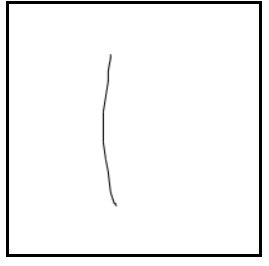
\includegraphics[scale=0.5]{./img/classificationexample}
	\end{subfigure}
	\caption{Example segment. $p_{vertex} = 0.0000076\text{, }   p_{arrow} = 0.256\text{, } p_{edge} = 0.996\text{, }  p_{loop} = 0.000086$}
	\label{fig:classification_example}
\end{figure}

%\subsection{Future Work}
%
%Our future work is to connect the probability distributions computed in this step to the domain interpretation step. Certain classes tend to have similar probabilities, for example, vertices and self-loops are difficult to differentiate. These are typically differentiated in domain interpretation rather than classification. \\
%
%In addition, we may need to further test these implementations on more data, or train more on our own data so that our weights better reflect our specific implementations.

